% Options for packages loaded elsewhere
\PassOptionsToPackage{unicode}{hyperref}
\PassOptionsToPackage{hyphens}{url}
%
\documentclass[
  12pt,
]{article}
\title{A comparative study of the corporate environmental impacts of the
six representative countries of six continents}
\usepackage{etoolbox}
\makeatletter
\providecommand{\subtitle}[1]{% add subtitle to \maketitle
  \apptocmd{\@title}{\par {\large #1 \par}}{}{}
}
\makeatother
\subtitle{\url{https://github.com/yw448/QiuWangXu_ENV872_EDA_FinalProject.git}}
\author{Ina, Qiu, Lehe, Xu, Yunting, Wang}
\date{}

\usepackage{amsmath,amssymb}
\usepackage{lmodern}
\usepackage{iftex}
\ifPDFTeX
  \usepackage[T1]{fontenc}
  \usepackage[utf8]{inputenc}
  \usepackage{textcomp} % provide euro and other symbols
\else % if luatex or xetex
  \usepackage{unicode-math}
  \defaultfontfeatures{Scale=MatchLowercase}
  \defaultfontfeatures[\rmfamily]{Ligatures=TeX,Scale=1}
  \setmainfont[]{Times New Roman}
\fi
% Use upquote if available, for straight quotes in verbatim environments
\IfFileExists{upquote.sty}{\usepackage{upquote}}{}
\IfFileExists{microtype.sty}{% use microtype if available
  \usepackage[]{microtype}
  \UseMicrotypeSet[protrusion]{basicmath} % disable protrusion for tt fonts
}{}
\makeatletter
\@ifundefined{KOMAClassName}{% if non-KOMA class
  \IfFileExists{parskip.sty}{%
    \usepackage{parskip}
  }{% else
    \setlength{\parindent}{0pt}
    \setlength{\parskip}{6pt plus 2pt minus 1pt}}
}{% if KOMA class
  \KOMAoptions{parskip=half}}
\makeatother
\usepackage{xcolor}
\IfFileExists{xurl.sty}{\usepackage{xurl}}{} % add URL line breaks if available
\IfFileExists{bookmark.sty}{\usepackage{bookmark}}{\usepackage{hyperref}}
\hypersetup{
  pdftitle={A comparative study of the corporate environmental impacts of the six representative countries of six continents},
  pdfauthor={Ina, Qiu, Lehe, Xu, Yunting, Wang},
  hidelinks,
  pdfcreator={LaTeX via pandoc}}
\urlstyle{same} % disable monospaced font for URLs
\usepackage[margin=2.54cm]{geometry}
\usepackage{graphicx}
\makeatletter
\def\maxwidth{\ifdim\Gin@nat@width>\linewidth\linewidth\else\Gin@nat@width\fi}
\def\maxheight{\ifdim\Gin@nat@height>\textheight\textheight\else\Gin@nat@height\fi}
\makeatother
% Scale images if necessary, so that they will not overflow the page
% margins by default, and it is still possible to overwrite the defaults
% using explicit options in \includegraphics[width, height, ...]{}
\setkeys{Gin}{width=\maxwidth,height=\maxheight,keepaspectratio}
% Set default figure placement to htbp
\makeatletter
\def\fps@figure{htbp}
\makeatother
\setlength{\emergencystretch}{3em} % prevent overfull lines
\providecommand{\tightlist}{%
  \setlength{\itemsep}{0pt}\setlength{\parskip}{0pt}}
\setcounter{secnumdepth}{5}
\ifLuaTeX
  \usepackage{selnolig}  % disable illegal ligatures
\fi

\begin{document}
\maketitle

\newpage
\tableofcontents 
\newpage
\listoftables 
\newpage
\listoffigures 
\newpage

\hypertarget{rationale-and-research-questions}{%
\section{Rationale and Research
Questions}\label{rationale-and-research-questions}}

As ESG performance became more and more important for investors to
measure a corporation's competitiveness, evaluating environmental
impacts of companies becomes an essential topic. Therefore, Harvard
Business School developed a methodology to monetize corporations'
environmental impacts. With the monetized impacts, we can measure the
overall environmental impacts of the corporations in a country.

Due to the different stages countries are in their industrial transition
path, different countries' corporations have different environmental
intensity. Therefore, by comparing the environmental intensity of the
representative countries in six continents, we can see which country's
corporations took the leading position in their way of industrial
transition. Since each country is the representative of its continent,
we can have an overview of the industrial transition status of the
world. The environmental intensity disparities of countries is also a
reminder for the laggards to perform better in the future.

Key Questions: Is there any countries better off than others 2019? Which
countries are better-off than others in 2019?

\newpage

\hypertarget{dataset-information}{%
\section{Dataset Information}\label{dataset-information}}

\textbf{1. Dataset Information}

The dataset we choose is from Harvard Business School's study of
corporate environmental impact. They develop a methodology to estimate
monetized environmental impact by ``applying characterization pathways
and monetization factors to organization level environmental outputs,
including carbon emissions, water use, and other emission types'' .
Their monetization factors are from ``the Environmental Priority
Strategies (EPS) Database, Available WAter REmaining (AWARE) Model, and
Waterfund, along with organization level data of environmental outputs,
such as carbon emissions, nitrous oxide, sulfur oxide, VOC, PM 2.5, and
water withdrawal and discharge, sourced from Bloomberg and Thomson
Reuters'' .

The monetized dataset includes Year, Company Name, Country, Industry,
Environmental Intensity (Sales), Environmental Intensity (Op Inc), Total
Environmental Cost, Capacity for each means of production, and the
monetized impact on each selected SDG goal. A total of 14516 rows are in
the dataset. The factor-environmental intensity (Sales) is the scaled
calculations for total organizational environmental impact by sales as a
proxy for organization size. The monetized damage to the environment is
minus, whereas the monetized benefits to the environment is plus. The
most recent year of data is 2019.

\newpage

\hypertarget{exploratory-analysis}{%
\section{Exploratory Analysis}\label{exploratory-analysis}}

\textbf{2. Data Wrangling} Our key research question is to compare the
corporate environmental impacts of the six representative countries of
six continents in 2019, because the data of 2019 is the most recent data
we have. The six representative countries are chosen for the countries
with the most environmental impacts data in their continents. Finally,
the US, UK, Japan, Australia, Mexico, and South Africa, these six
countries was selected.

The main effect variable we want to discuss is ``Environmental Intensity
(Sales)'', so we deleted all the irrelevant variables, and only left
``Year'', ``Company'', ``Country'', and ``Environmental Intensity
(Sales)''-these four columns.

To make the graph easier to read, we multiplied ``Environmental
Intensity (Sales)'' by ``-1'', so that the larger the number is, the
larger negative impacts the environment are suffered.

\begin{verbatim}
##            Argentina            Australia              Austria 
##                   18                  584                   94 
##              Bahrain              Belgium              Bermuda 
##                    1                   63                   13 
##               Brazil               Canada                Chile 
##                  136                  411                   44 
##                China             Colombia              Croatia 
##                  241                   36                    9 
##       Czech Republic              Denmark        Faeroe Island 
##                   10                   71                    1 
##              Finland               France              Georgia 
##                  124                  565                    6 
##              Germany            Gibraltar               Greece 
##                  389                    3                   43 
##             Guernsey            Hong Kong              Hungary 
##                    6                  319                   21 
##                India            Indonesia              Ireland 
##                  239                   19                   67 
##          Isle of Man               Israel                Italy 
##                    9                   18                  164 
##                Japan               Jersey                Kenya 
##                 2401                    3                    5 
##               Kuwait           Luxembourg                Macau 
##                    8                   17                    8 
##             Malaysia                Malta               Mexico 
##                   98                    5                  193 
##              Morocco          Netherlands          New Zealand 
##                    3                  187                   29 
##               Norway                 Oman             Pakistan 
##                  111                    3                    6 
##                 Peru          Philippines               Poland 
##                    2                   86                   35 
##             Portugal                Qatar              Romania 
##                   57                    5                   11 
##               Russia         Saudi Arabia            Singapore 
##                   77                    5                  134 
##             Slovenia         South Africa          South Korea 
##                    1                  527                  533 
##                Spain            Sri Lanka               Sweden 
##                  248                   16                  324 
##          Switzerland               Taiwan             Thailand 
##                  378                 1024                  102 
##               Turkey              Ukraine United Arab Emirates 
##                   51                    2                    8 
##       United Kingdom        United States 
##                 1691                 2397
\end{verbatim}

\textbf{3. Data Exploration}

\begin{verbatim}
## [1] 7793    4
\end{verbatim}

\begin{verbatim}
##       Year                           Company               Country    
##  2017   : 895   3M COMPANY               :  10   Japan         :2401  
##  2016   : 888   ABSA GROUP LTD           :  10   United States :2397  
##  2018   : 830   ADELAIDE BRIGHTON LIMITED:  10   United Kingdom:1691  
##  2019   : 815   ADVANTEST CORPORATION    :  10   Australia     : 584  
##  2015   : 804   AEON MALL COMPANY LIMITED:  10   South Africa  : 527  
##  2014   : 795   AGC INC                  :  10   Mexico        : 193  
##  (Other):2766   (Other)                  :7733   (Other)       :   0  
##      Index          
##  Min.   :-1.390194  
##  1st Qu.: 0.006238  
##  Median : 0.017521  
##  Mean   : 0.107617  
##  3rd Qu.: 0.074098  
##  Max.   : 1.992787  
## 
\end{verbatim}

\begin{verbatim}
## `summarise()` has grouped output by 'Country'. You can override using the `.groups` argument.
\end{verbatim}

\begin{verbatim}
## `geom_smooth()` using formula 'y ~ x'
\end{verbatim}

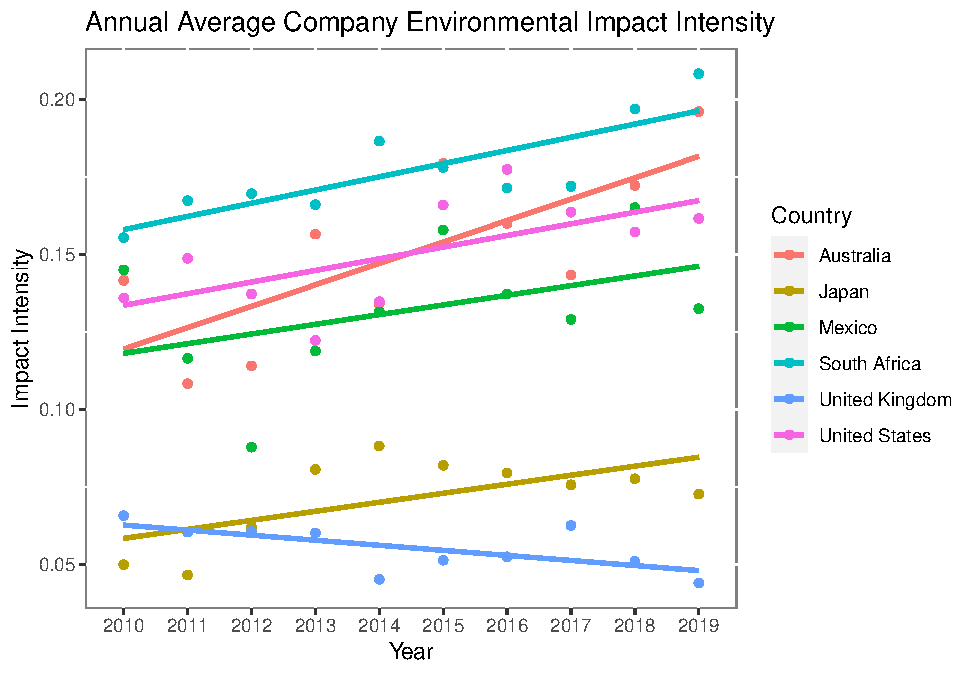
\includegraphics{QiuWangXu_ENV872_Finalproject_files/figure-latex/unnamed-chunk-3-1.pdf}
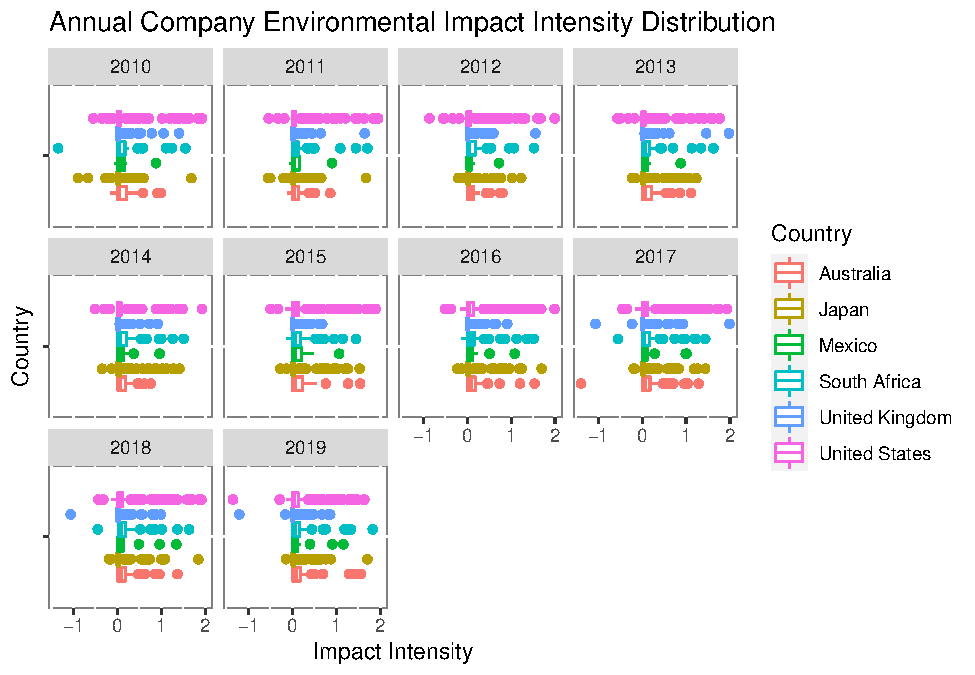
\includegraphics{QiuWangXu_ENV872_Finalproject_files/figure-latex/unnamed-chunk-3-2.pdf}

\newpage

\hypertarget{analysis}{%
\section{Analysis}\label{analysis}}

\begin{verbatim}
## 
##  Shapiro-Wilk normality test
## 
## data:  Year2019$Index[Year2019$Country == "Australia"]
## W = 0.5764, p-value = 6.644e-13
\end{verbatim}

\begin{verbatim}
## 
##  Shapiro-Wilk normality test
## 
## data:  Year2019$Index[Year2019$Country == "Japan"]
## W = 0.42944, p-value < 2.2e-16
\end{verbatim}

\begin{verbatim}
## 
##  Shapiro-Wilk normality test
## 
## data:  Year2019$Index[Year2019$Country == "South Africa"]
## W = 0.56954, p-value = 4.133e-11
\end{verbatim}

\begin{verbatim}
## 
##  Shapiro-Wilk normality test
## 
## data:  Year2019$Index[Year2019$Country == "United Kingdom"]
## W = 0.45052, p-value < 2.2e-16
\end{verbatim}

\begin{verbatim}
## 
##  Shapiro-Wilk normality test
## 
## data:  Year2019$Index[Year2019$Country == "United States"]
## W = 0.60069, p-value < 2.2e-16
\end{verbatim}

\begin{verbatim}
## 
##  Shapiro-Wilk normality test
## 
## data:  Year2019$Index[Year2019$Country == "Mexico"]
## W = 0.52411, p-value = 2.986e-08
\end{verbatim}

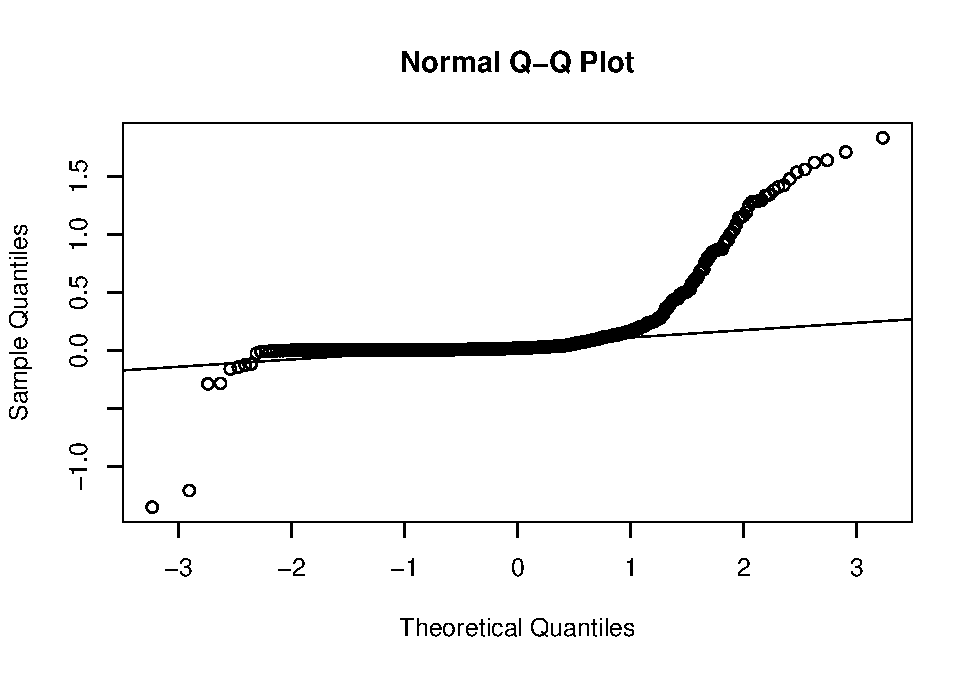
\includegraphics{QiuWangXu_ENV872_Finalproject_files/figure-latex/unnamed-chunk-5-1.pdf}

\begin{verbatim}
## 
##  Bartlett test of homogeneity of variances
## 
## data:  Year2019$Index by Year2019$Country
## Bartlett's K-squared = 213.26, df = 5, p-value < 2.2e-16
\end{verbatim}

\begin{verbatim}
##              Df Sum Sq Mean Sq F value Pr(>F)    
## Country       5   2.79  0.5578   7.373  9e-07 ***
## Residuals   809  61.21  0.0757                   
## ---
## Signif. codes:  0 '***' 0.001 '**' 0.01 '*' 0.05 '.' 0.1 ' ' 1
\end{verbatim}

\begin{verbatim}
## $statistics
##      MSerror  Df      Mean      CV
##   0.07565801 809 0.1153906 238.373
## 
## $parameters
##    test  name.t ntr StudentizedRange alpha
##   Tukey Country   6         4.039786  0.05
## 
## $means
##                     Index       std   r          Min       Max         Q25
## Australia      0.19612327 0.3483305  70 -0.001497662 1.5583389 0.014773036
## Japan          0.07270127 0.1741734 234 -0.143046024 1.7091834 0.007539765
## Mexico         0.13254267 0.2769682  27 -0.024868665 1.1622471 0.004186873
## South Africa   0.20834417 0.3903786  52  0.001405651 1.8321458 0.016665110
## United Kingdom 0.04403163 0.1576510 178 -1.207315335 0.8622585 0.002090376
## United States  0.16162368 0.3534198 254 -1.350964518 1.6380528 0.007599951
##                        Q50        Q75
## Australia      0.068164944 0.17916116
## Japan          0.016284642 0.04954285
## Mexico         0.033507035 0.11986662
## South Africa   0.038476424 0.16808371
## United Kingdom 0.007530084 0.02637540
## United States  0.024853952 0.13522728
## 
## $comparison
## NULL
## 
## $groups
##                     Index groups
## South Africa   0.20834417      a
## Australia      0.19612327      a
## United States  0.16162368      a
## Mexico         0.13254267     ab
## Japan          0.07270127      b
## United Kingdom 0.04403163      b
## 
## attr(,"class")
## [1] "group"
\end{verbatim}

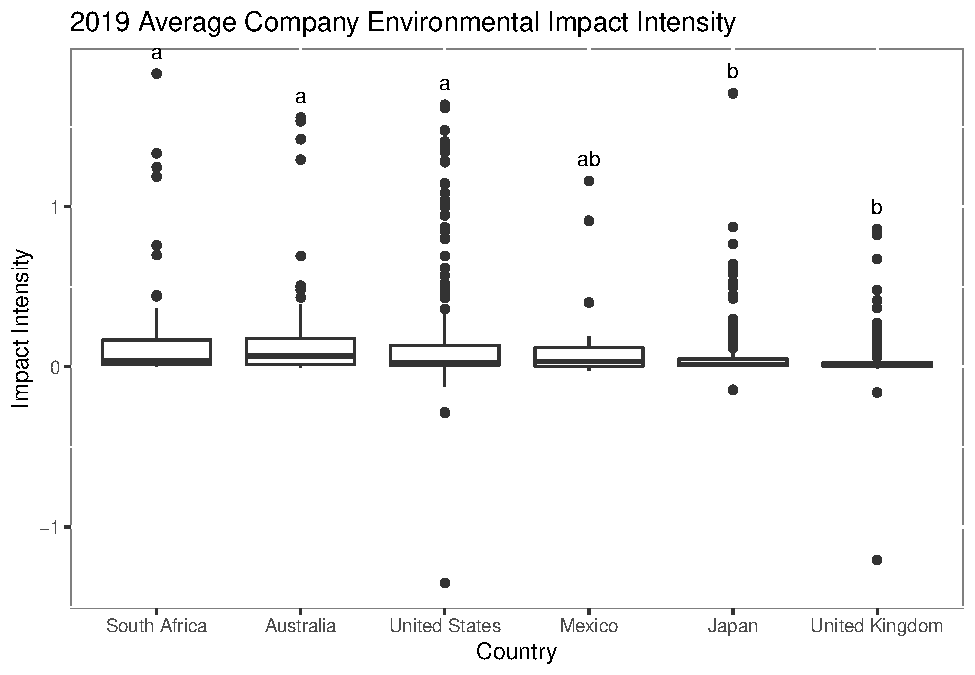
\includegraphics{QiuWangXu_ENV872_Finalproject_files/figure-latex/unnamed-chunk-6-1.pdf}

\hypertarget{question-1-is-there-any-countries-better-off-than-others}{%
\subsection{Question 1: \textless Is there any countries better off than
others?
\textgreater{}}\label{question-1-is-there-any-countries-better-off-than-others}}

Answer:

\hypertarget{question-2-which-countries-are-better-off-than-others}{%
\subsection{Question 2: \textless Which countries are better-off than
others?\textgreater{}}\label{question-2-which-countries-are-better-off-than-others}}

Answer:

\newpage

\hypertarget{summary-and-conclusions}{%
\section{Summary and Conclusions}\label{summary-and-conclusions}}

\begin{verbatim}
## `summarise()` has grouped output by 'industry'. You can override using the `.groups` argument.
\end{verbatim}

\newpage

\hypertarget{references}{%
\section{References}\label{references}}

\textless Freiberg, et. al.~2020, Corporate Environmental Impact:
Measurement, Data, and Information, Harvard Business School,
Impact-Weighted Accounts Project Research Report. Retrieved from:
\url{https://www.hbs.edu/impact-weighted-accounts/Documents/corporate-environmental-impact.pdf}\textgreater{}

\end{document}
